\documentclass[fleqn]{article}
\usepackage{graphicx}

\usepackage{haldefs}
\usepackage{notes}
\usepackage{url}

\begin{document}
\lecture{Machine Learning}{HW02: Clustering and perceptrons}{Angjoo
  Kanazawa(Kim), UID:111964222}

% IF YOU ARE USING THIS .TEX FILE AS A TEMPLATE, PLEASE REPLACE
% "CS 726, Fall 2011" WITH YOUR NAME AND UID.

Hand in at: \url{http://www.cs.utah.edu/~hal/handin.pl?course=cs726}.
Remember that only PDF submissions are accepted.  We encourage using
\LaTeX\ to produce your writeups.  See \verb+hw00.tex+ for an example
of how to do so.  You can make a \verb+.pdf+ out of the \verb+.tex+ by
running ``\verb+pdflatex hw00.tex+''.

\begin{enumerate}
\item Give an example of a low dimensional (approx 20 dimensions), a
  medium dimensional (approx 1000 dimensions) and a high dimensional
  (approx 100000 dimensional) problem that you care about.

\begin{solution}
  Low dimensional: spam filtering. Using existence of 10 keywords
  (binary yes no val for each)

  Medium dimensional:Optical character recognition on digits
  representing each digit with 100x100 grid pixel values

  High dimensional:  Identifying cats on images using high dimensional feature vector to represent cats.
\end{solution}  

\item What does the decision boundary for a one nearest neighbor
  classifier on two data points (one positive, one negative) look
  like?

\begin{solution}
  It will be a linear line since the data is seperable by a single line.
\end{solution}  

\item (Final book question from chapter 2.)  Clustering of classes was
  introduced as a way of making things faster.  Will it make things
  worse, or could it help?

\begin{solution}
  Clustering will help if it's done correctly, correctly as in the
  optimal way to feed it to the algorithm. Clustering could make
  things worse if the clustering is not done well. i.e. data maybe
  clustered on features that we don't care about.
\end{solution}  

\item A common way to get rid of having to deal with the bias
  separately on a perceptron is to add a new feature.  This feature
  always has value one, and you learn a weight for it.  Thus, if you
  have a $100$ dimensional problem with a bias, we solve it as a $101$
  dimensional problem without a bias.  Draw a picture for \emph{one
    dimensional} data and a linear separator with a (non-zero) bias
  and draw the corresponding picture for the same data, ``lifted''
  into two dimensions, with the corresponding lineear separate
  \emph{without} a bias.  (Please make sure that the two separators
  are actually \emph{equiavalent}!)
\pagebreak
\begin{solution}
%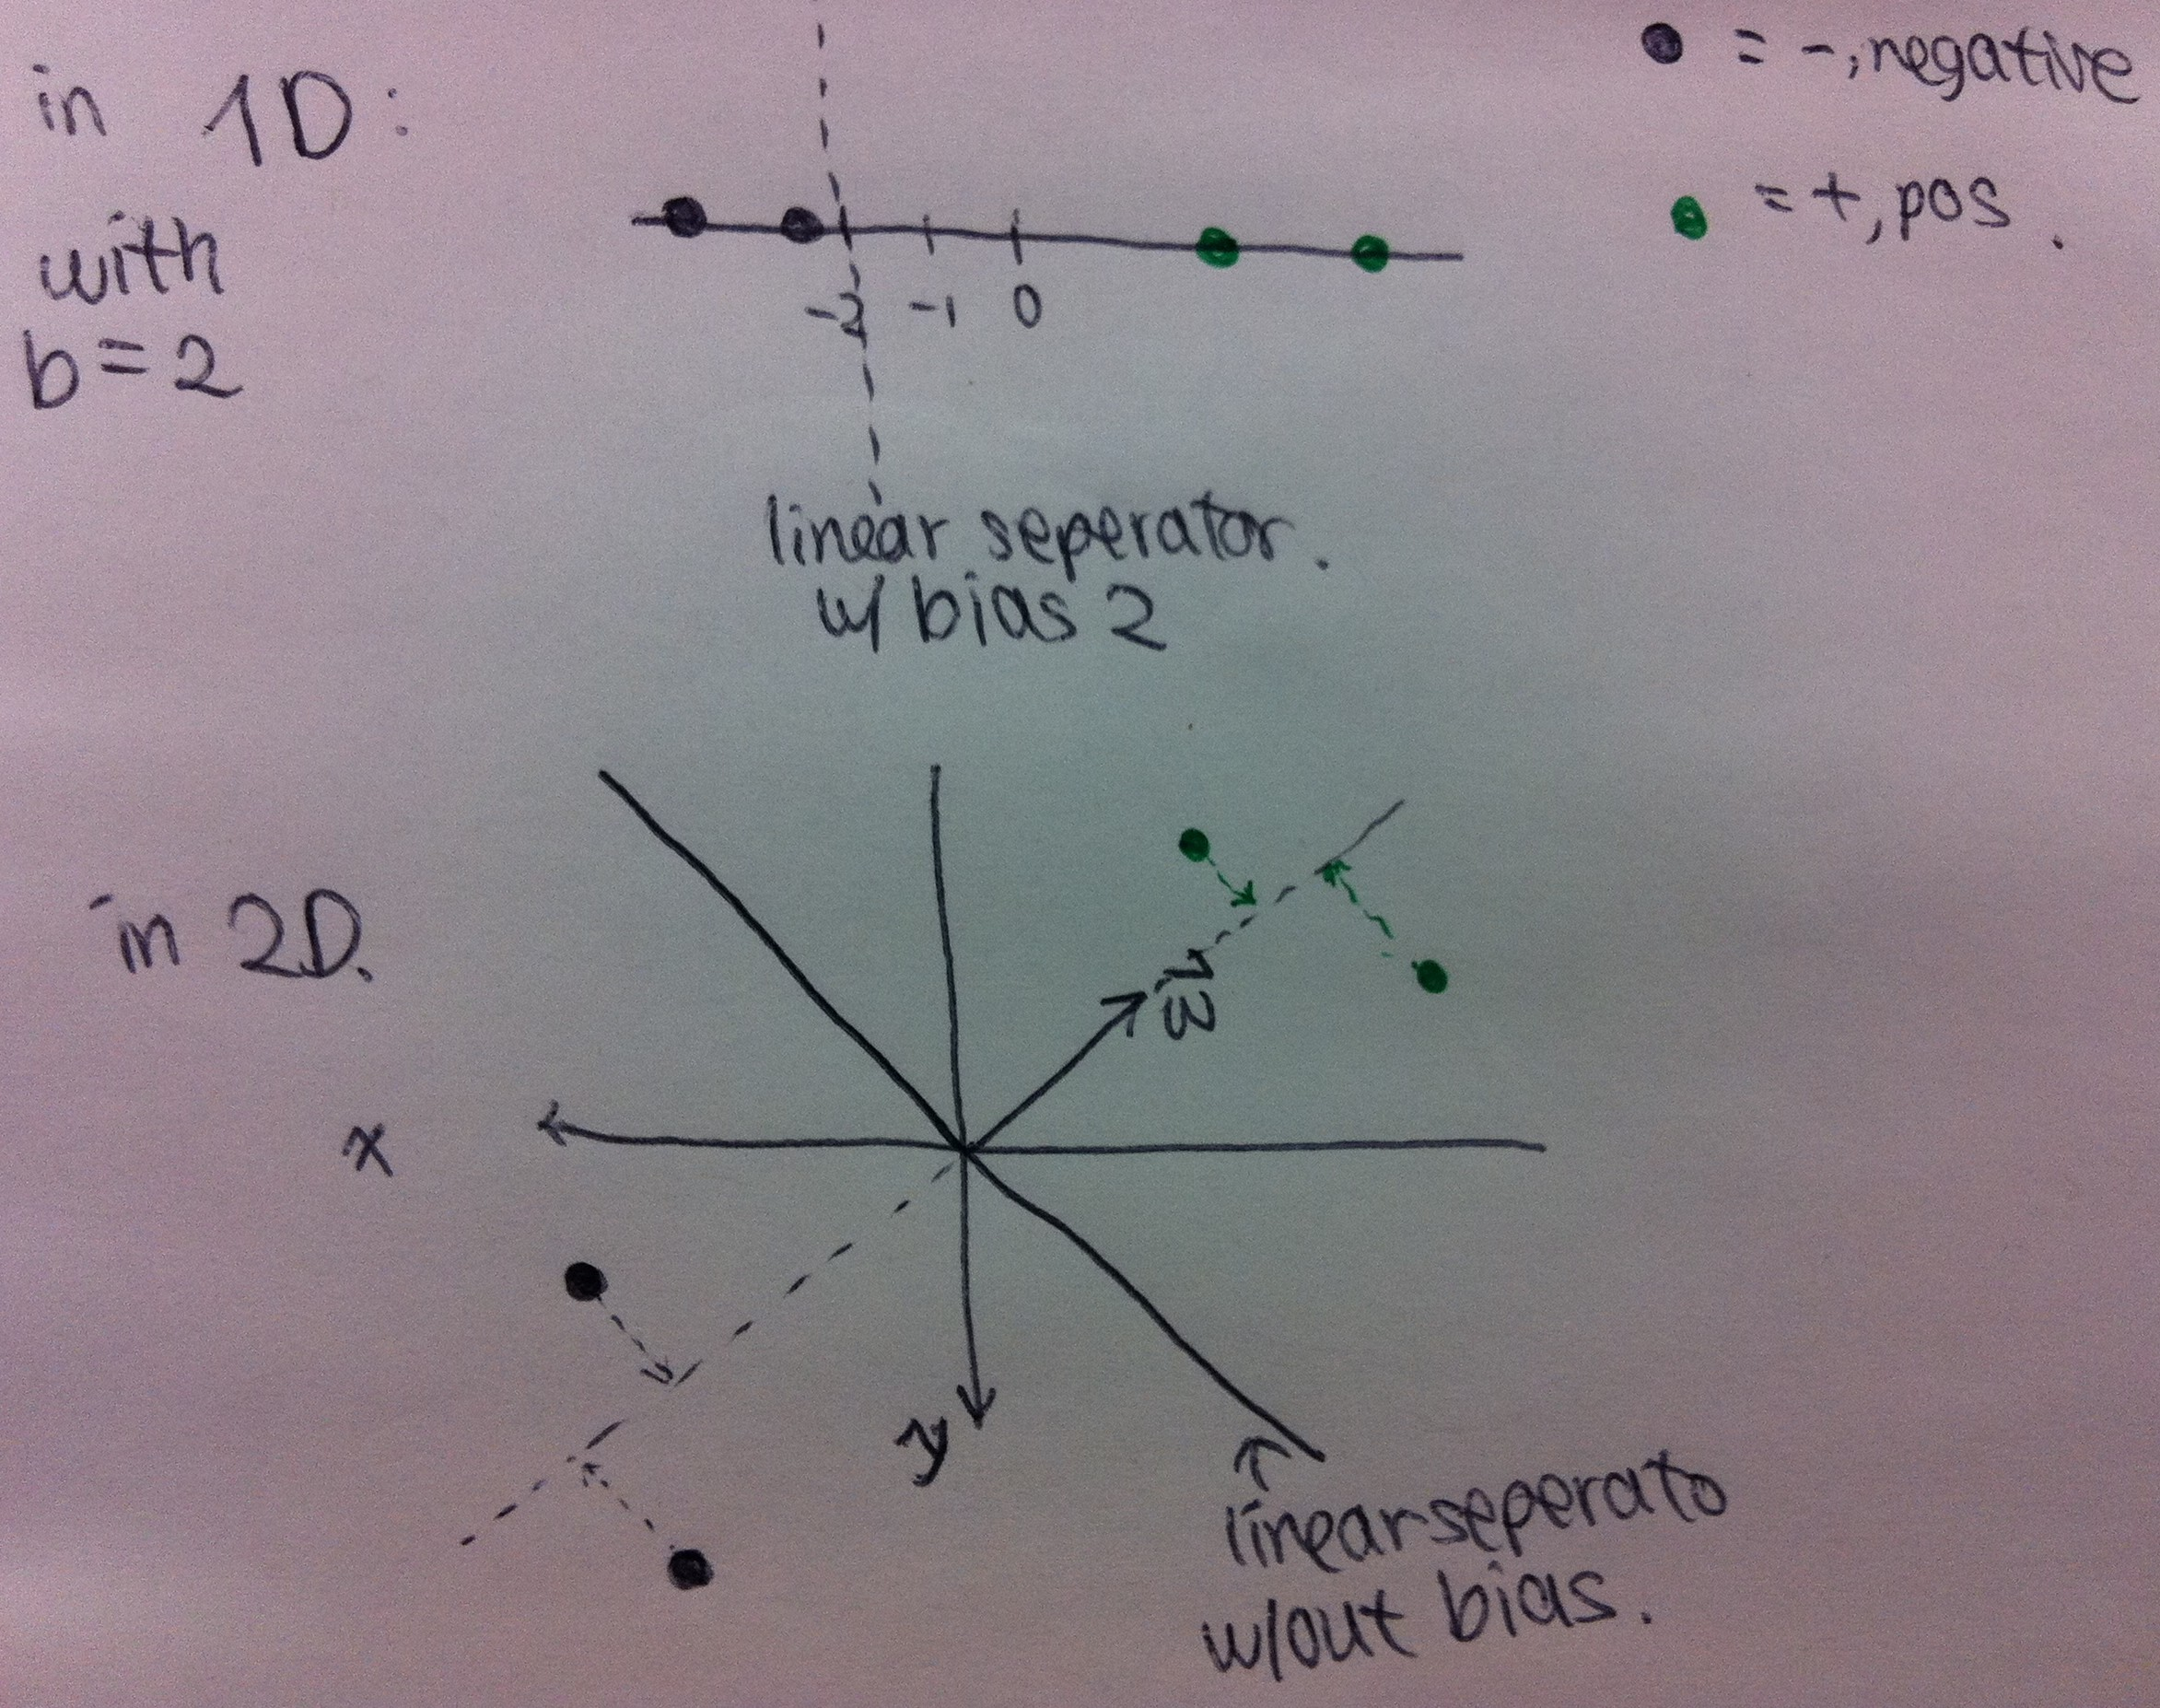
\includegraphics[scale=0.2,bb=0 0 500 500]{fig1.png}
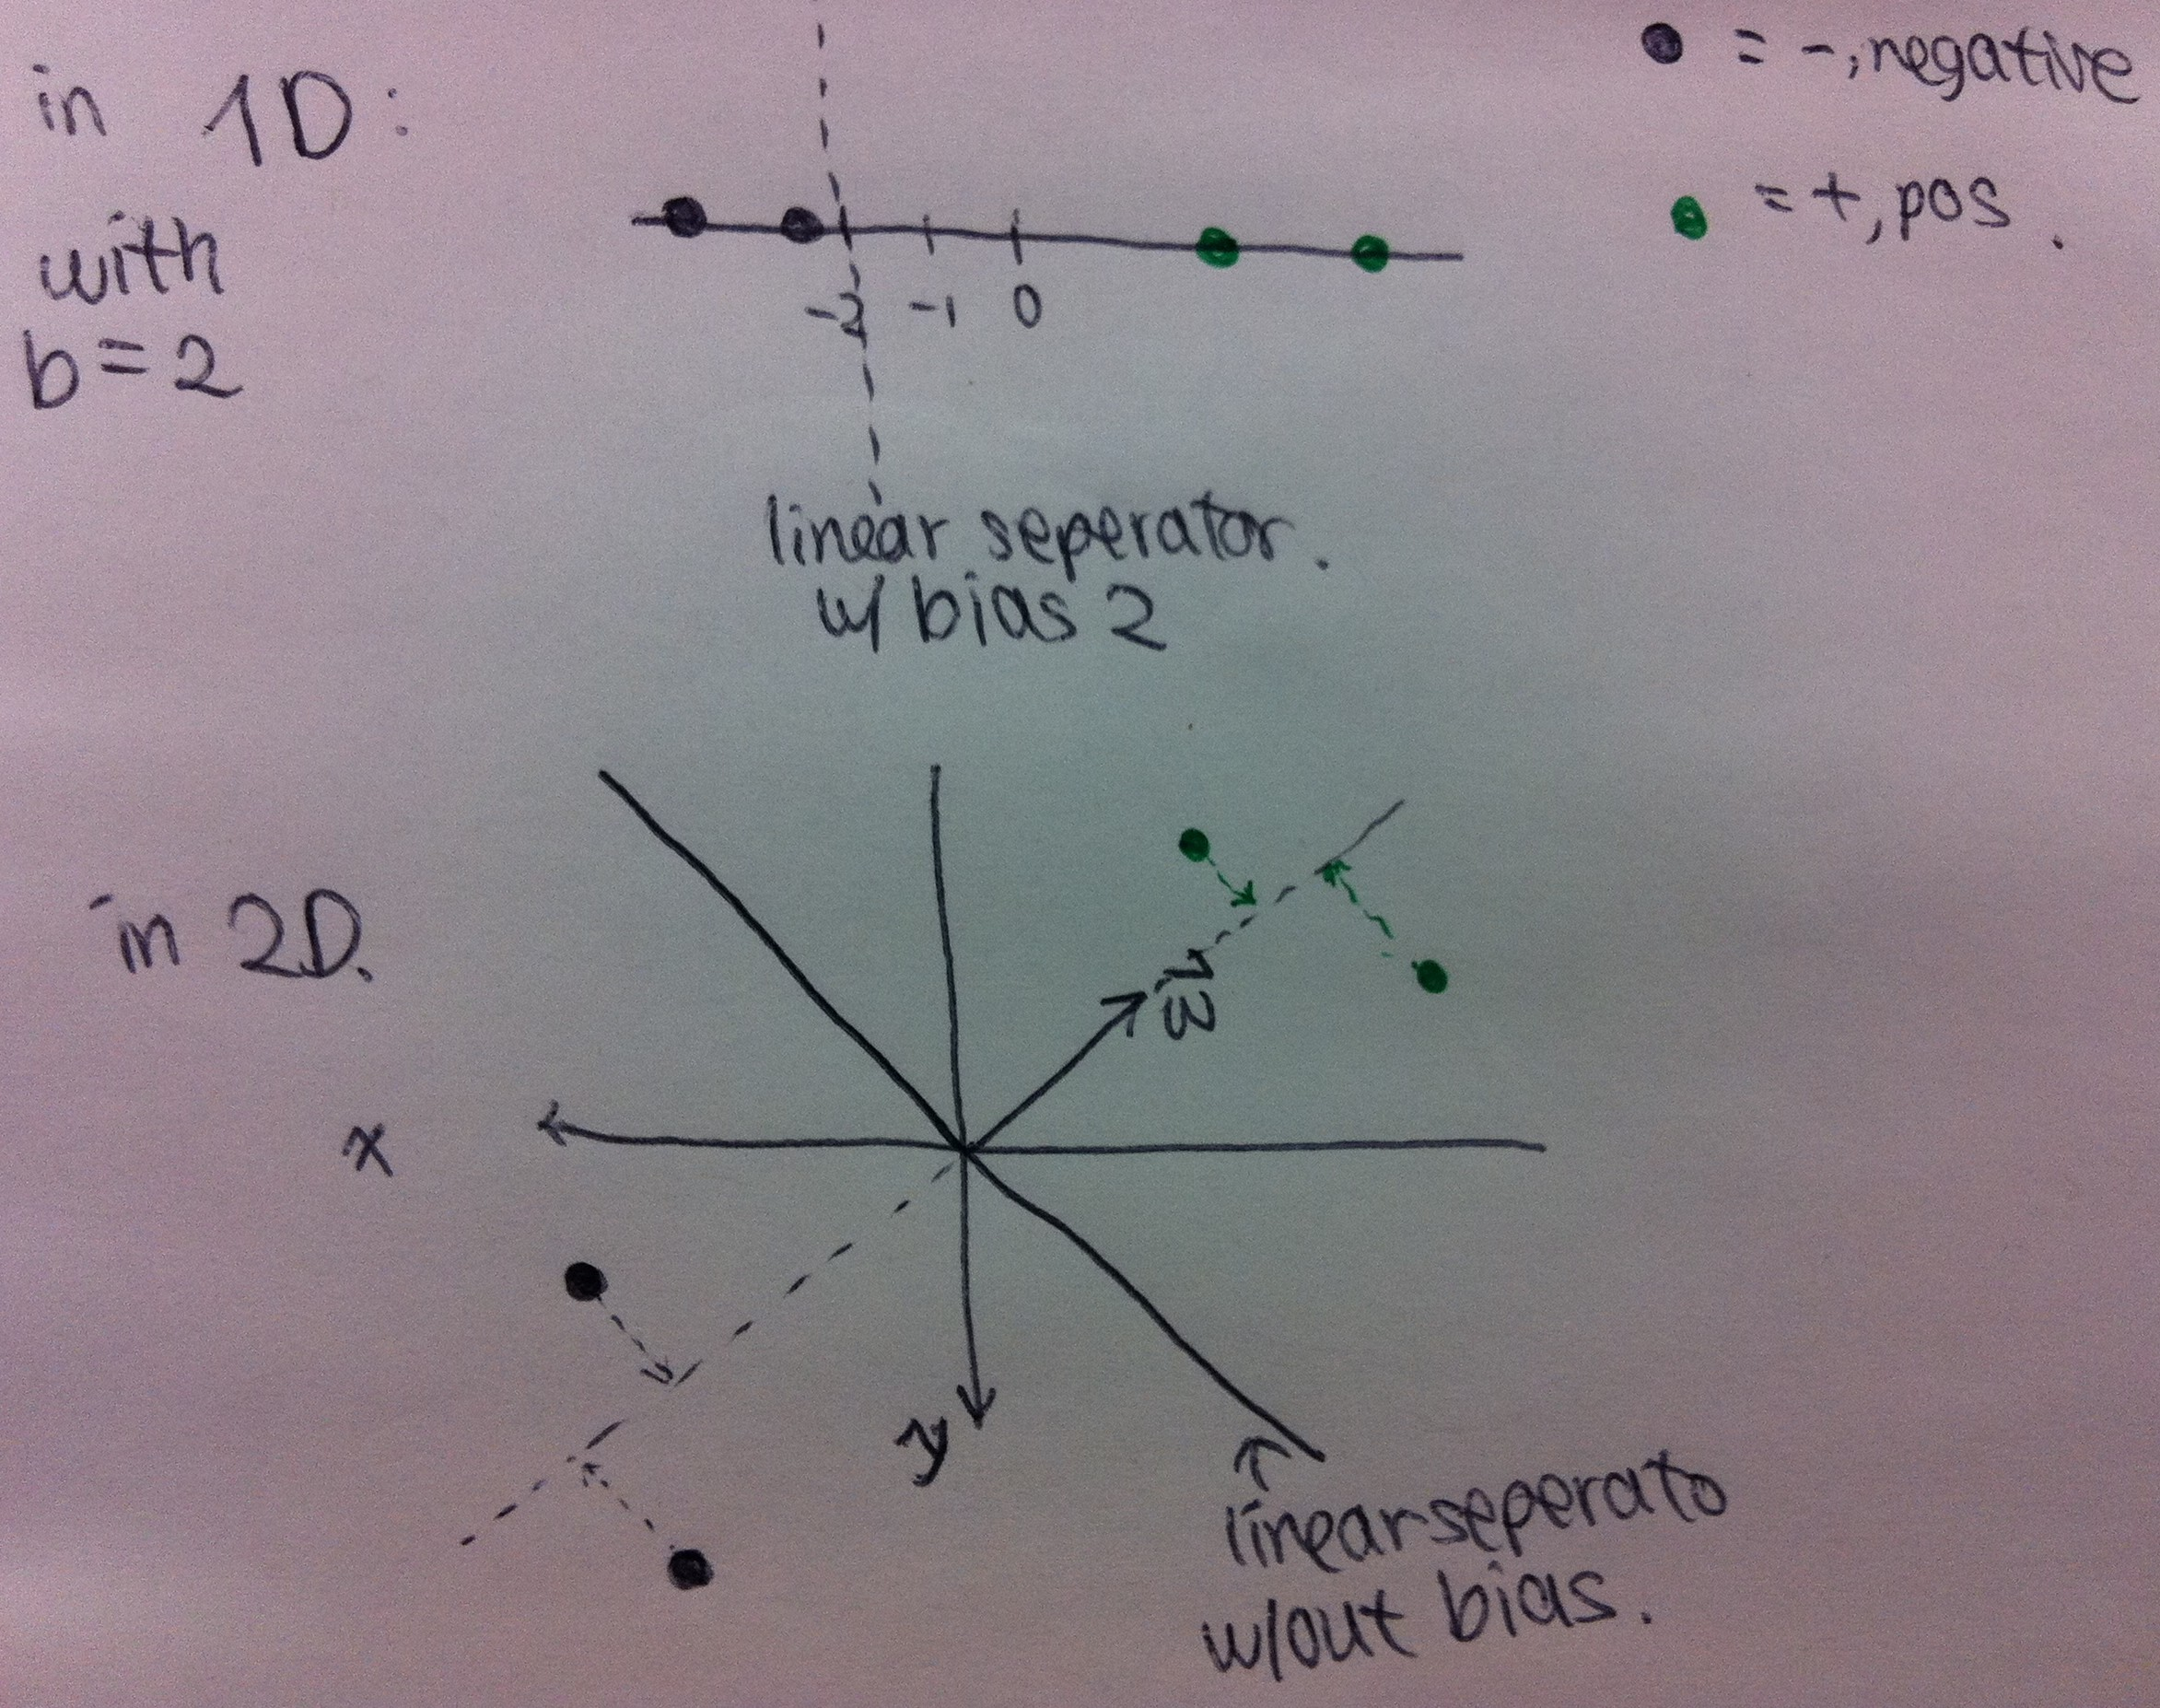
\includegraphics[scale=0.2]{fig1.png}
\end{solution}  

\end{enumerate}

\end{document}
